\documentclass{beamer}
\usepackage{amsmath}
\usepackage{amssymb}
\usepackage{pgf}
\usepackage{tikz}
\usetikzlibrary{matrix}
\usetheme{boxes}
\newcommand{\fig}{figures} % common figure path
\newcommand{\frnzplt}{FranzPlot }
\newcommand{\dbbslsh}{\textbackslash \textbackslash} % common figure path
\title[Curve e Sup. - Lab 2]{Curve e Superfici per il Design \\ Laboratorio - 2}
\author[Prof.ssa Scotti]{Prof.ssa Anna Scotti}
%\institute[dimat]{Long Inst.}
\date{9 Aprile 2019}

\begin{document}
\begin{frame}
\maketitle
\end{frame}
\begin{frame}
\frametitle{Materiali}
Nella cartella su beep con il materiale di oggi troverete:
\begin{itemize}
\item Questa presentazione (\texttt{lab2.pdf});
\item Il file \texttt{es\_dado\_ref.toml} con l'esercizio risolto della passata esercitazione.
\end{itemize}
Nella cartella `Materiale Laboratorio' (sempre su Beep) troverete:
\begin{itemize}
\item Un riferimento con indicate le trasformazioni (Rotazione, scaling taglio etc.): \texttt{trasformazioni\_ref.pdf};
\item Eventuali pdf con risoluzioni di esercizi ed esercizi risolti
\end{itemize}
\end{frame}
\begin{frame}
\frametitle{Coordinate omogenee}
\begin{displaymath}
\begin{bmatrix}
a_{11} & a_{12} & a_{13} & t_1 \\
a_{21} & a_{22} & a_{23} & t_2 \\
a_{31} & a_{32} & a_{33} & t_3 \\
0      &    0   &  0     & 1 
\end{bmatrix}
~\begin{bmatrix}
x \\ y\\ z\\ 1
\end{bmatrix}
=  
\begin{bmatrix}
a_{11}x + a_{12}y + a_{13}z + t_1 \\
a_{21}x + a_{22}y + a_{23}z + t_2 \\
a_{31}x + a_{32}y + a_{33}z + t_3 \\
 1
\end{bmatrix}
\end{displaymath}
\end{frame}

\section{Esercizi}
%
\begin{frame}
\frametitle{Esercizio 1 - I}
\begin{itemize}
\item Disegnare un cilindro con asse parallelo a z, raggio 0.6, altezza 1 e centro di una base nell'origine.
\item Ruotare l'oggetto cos\`i ottenuto di $60^\circ$ intorno all'asse y e traslarlo di un vettore 
$( 1,0,1)$, calcolando la corrispondente matrice di trasformazione composta.
\item Applicare rotazione e traslazione invertendo l'ordine e provare che la composizione non commuta.
\end{itemize}
\end{frame}
\begin{frame}
\frametitle{Esercizio 1 - II}
\begin{center}
\begin{tikzpicture}
\node(img1){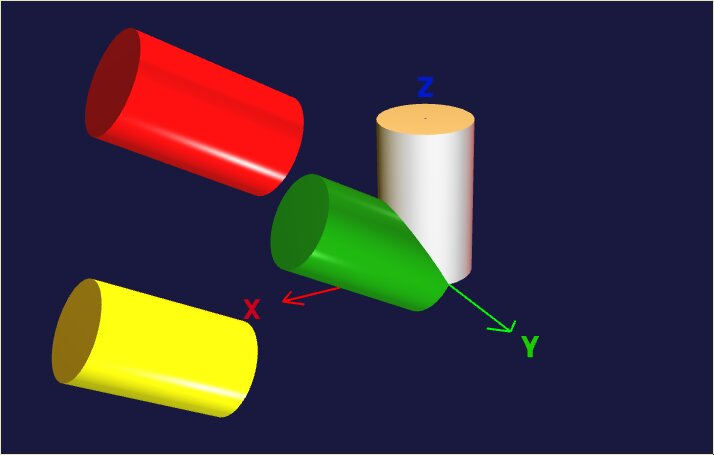
\includegraphics[width=0.6\textwidth]{\fig/l2_es1_c.jpeg}};
\node(img2) at (img1.south east){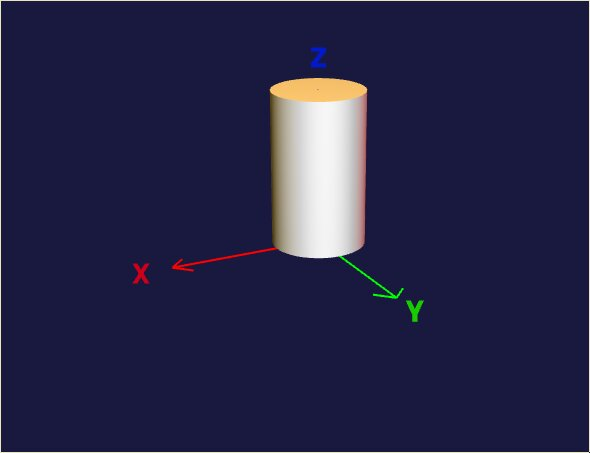
\includegraphics[width=0.3\textwidth]{\fig/l2_es1_a.jpeg}};
\end{tikzpicture}
\end{center}
\begin{block}{Per casa}{Risolvere lo stesso esercizio componendo un'unica matrice (quindi aggiungendo lo scaling e la traslazione iniziale )}
\end{block}
\end{frame}

\begin{frame}
\frametitle {Esercizio 2-I}
\begin{itemize}
\item Creare un oggetto 'dado' utilizzando il comando Primitive, con fattore di
scala 0.5 e traslare il centro dell'oggetto in   $( 2,1,0)^T$. 
\item Ruotare l'oggetto di 180 gradi rispetto all'asse $\langle -1,1,0 \rangle$.
\item Rappresentare il dado, il dado ruotato e l'asse di rotazione con \frnzplt
\item Che differenze si osservano tra il risultato di questo esercizio con il precedente?

\end{itemize}
\end{frame}
\begin{frame}
\frametitle{ Esercizio 2-II}
La caratteristica principale di questo esercizio \`e di richiedere una
rotazione su un asse che non corrisponde ad uno dei tre assi cartesiani, e del
quale, quindi, non abbiamo a disposizione una formula in
\texttt{trasformazioni\_ref.pdf}.\\ 
La strategia di risoluzione consiste nel
comporre tre rotazioni:
\begin{enumerate}
\item Un prima trasformazione servir\`a a portare l'asse di rotazione in corrispondenza di un asse cartesiano;
\item La seconda trasfomazione eseguir\`a la rotazione richiesta dall'esercizio;
\item La terza rotazione sar\`a l'inversa della prima e servir\`a a riportare l'asse nella posizione originaria.
\end{enumerate}
\end{frame}
\begin{frame}
\frametitle{Esercizio 2-III}
\begin{itemize}
\item L'asse di rotazione giace sul piano $xy$ ed il suo angolo con l'asse y,
calcolabile utilizzando le definizioni del prodotto scalare, \`e di
-45$^\circ$.  
\item Si tratta quindi di eseguire una rotazione di -45$^\circ$ rispetto a z,
una rotazione di 180$^\circ$ rispetto ad y, ed infine di ruotare di 45$^\circ$ di nuovo
rispetto a z.  
\end{itemize}
Utilizzando le definizioni che abbiamo a disposizione otteniamo:
%
\begin{displaymath}
R(180^\circ)_{(1,1,0)}= R(-45^\circ)_z~R(180^\circ)_y~R(45^\circ)=
\end{displaymath}
\begin{displaymath}
\begin{bmatrix}
\frac{\sqrt{2}}{2}  & -\frac{\sqrt{2}}{2} & 0 \\
\frac{\sqrt{2}}{2} &  \frac{\sqrt{2}}{2}& 0 \\ 
0  &  0 & 1 
\end{bmatrix}
\begin{bmatrix}
-1  & 0   & 0 \\
0   & -1  & 0 \\ 
0   &  0  & 1 
\end{bmatrix}
\begin{bmatrix}
\frac{\sqrt{2}}{2}  & \frac{\sqrt{2}}{2} & 0 \\
-\frac{\sqrt{2}}{2} &  \frac{\sqrt{2}}{2}& 0 \\ 
0  &  0 & 1 
\end{bmatrix}
{\color[rgb]{0.1,0,1}
=
\begin{bmatrix}
0  & -1 & 0 \\
-1 &  0 & 0 \\ 
0  &  0 & -1 
\end{bmatrix}
}
\end{displaymath}
\end{frame}

\begin{frame}
\frametitle{Esercizio 2-iv}
\begin{center}
\begin{tikzpicture}
\node(img1){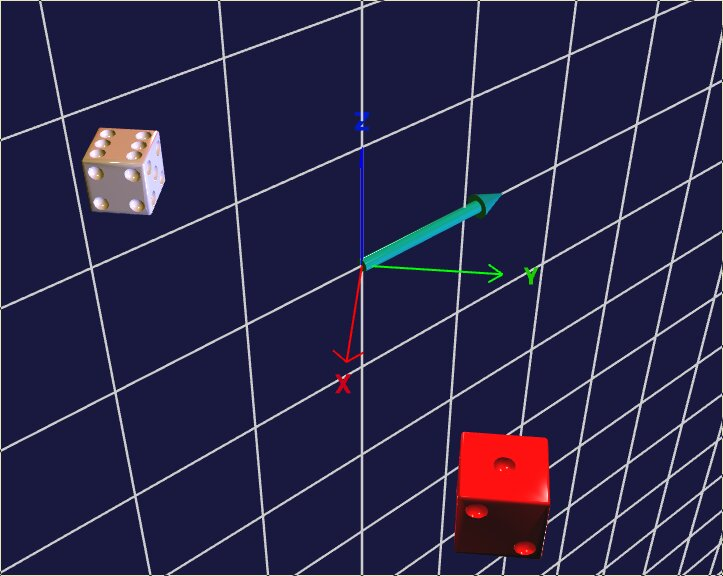
\includegraphics[width=0.7\textwidth]{\fig/l2_es2_dadorot.jpeg}};
%\node(img2) at (img1.north east){\includegraphics[width=0.4\textwidth]{\fig/snapcode_3-4.png}};
\end{tikzpicture}
\end{center}
\end{frame}
\begin{frame}
\frametitle{Esercizio 3}
\begin{itemize}
\item Si consideri una sfera di raggio 0.5, con centro nel punto $C=(1,0,0)$. Si
considerino la matrice di scaling $\mathcal{S}$ con $S_x=2$ $S_y=1$ ed $S_z =0.5$ e la matrice 
\begin{displaymath}
\mathcal{B} =  \begin{bmatrix}
                0 & 0 & 1\\
                0  & 1 & 0\\
                -1 & 0 & 0
                \end{bmatrix}
\end{displaymath}
\item Si applichi alla sfera prima la trasformazione $\mathcal{S}$ e poi la trasformazione $\mathcal{B}$.
\item Si applichi alla sfera prima la trasformazione $\mathcal{B}$ e poi la trasformazione $\mathcal{S}$.
\item Le trasformazioni $\mathcal{B}$ ed $\mathcal{S}$ commutano?
\item Che tipo di trasformazione \`e $\mathcal{B}$?
\end{itemize}
\end{frame}
\begin{frame}
\frametitle{Esercizio 3}
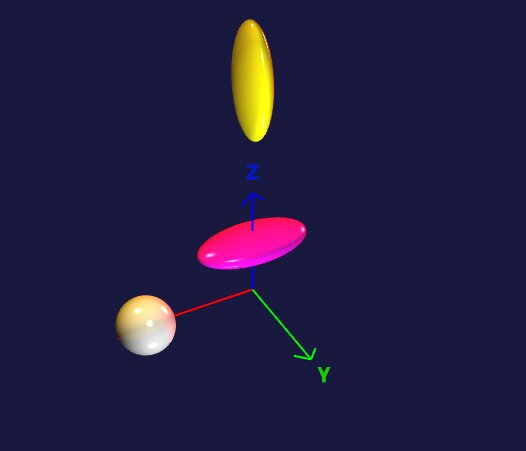
\includegraphics[width=0.9\textwidth]{\fig/l2_es3.jpeg}
\end{frame}
%


\end{document}
